\chapter{Query Context Selection}

% better name
% L  Local 
% QC Query Context 
% ET Expansion Term
% R  Refinement
% S  Selection

%\section{Natural Disambiguation}

% And not just the literal semantics of the words, but also the delivery, and inflection, the context of the occurrence of the statement, the social context, the political context, 

% Natural effortless disambiguation

Is it possible to have a context-free word? As my Dad always says:

\begin{center}
    \centering
    \textit{``Yes''}
\end{center}

The human mind can disambiguate the meaning of individual words by accounting for the wider context. For example, in the Oxford English Dictionary, \textit{``set''} has over 430 definitions making it the most polysemous word in the English language. However, within the context of the sentence \textit{``we must set out before dawn''} it does not seem ambiguous to me. A fluent reader can naturally disambiguate with amazing cognitive ease through the semantics of the other words and the surrounding grammar. You are doing it now; look at you go!

Here is an easier example to explain. In the following four sentences, can you assign a single word sense to each occurrence of \textit{``bank''}?

\begin{enumerate}
    \item \textit{``It's a \textbf{bank}.''}
    \item \textit{``They made all of their profits from the rushes on the \textbf{banks}''}
    \item \textit{``I saw three bears by the river \textbf{bank}.''}
    \item \textit{``I was \textbf{banking}\textsubscript{1} on the aeroplane to \textbf{bank}\textsubscript{2} into the river \textbf{bank}\textsubscript{3}, for I had over insured it with my \textbf{bank}\textsubscript{4}''}
\end{enumerate}

The first is impossible as it is too vague, it lacks context. The second is also impossible as it is a pun, the context is overloaded. Number three is just right\footnote{...said Goldilocks before being mauled in the face by a territorial mother bear}. The fourth sentence is an antanaclasis and contains 4 occurrences of the word ``bank''. Each can be disambiguated by considering the the context; the words preceding and following the term of interest. For example, \textit{bank}\textsubscript{3} is preceded by the attributive noun \textit{river}, which is preceded by the determiner \textit{the}. So the word sense of \textit{bank}\textsubscript{3} is clearly the land alongside a river. Table \ref{bank-definitions} shows all four intended definitions in the antanaclasis.

% Restricted expansion of query terms using part of speech tagging
% https://patents.google.com/patent/US5721902A/en

\begin{table}[h]
\centering
\begin{tabular}{|l|l|l|}
\hline
Term    & Part of speech & Definition                          \\ \hline
\textbf{\textit{bank on}}\textsubscript{1} & phrasal verb & To rely on confidently.             \\
\textbf{\textit{bank}}\textsubscript{2}    & noun & The land alongside a river or lake. \\
\textbf{\textit{bank}}\textsubscript{3}    & verb & To tilt sideways in making a turn.  \\
\textbf{\textit{bank}}\textsubscript{4}    & noun & A financial establishment.          \\ \hline
\end{tabular}
\caption{Four (of 18) Possible Definitions of the Term \textit{bank}}
\label{bank-definitions}
\end{table}

% It should be clear that polysemes (and homographs) can be naturally disambiguated using the other words in the sentence.

\section{Na{\"i}ve Expansion Selection} \label{standardTS}
The na{\"i}ve approach to query expansion with a semantic ontology is to include \textit{\textbf{all}} the provided candidate expansions without restriction. This is problematic since it is unlikely that a single query term refers to more than a single word sense. This problem becomes apparent when considering polysemes (and homographs). For example, if one were expanding the query term \textit{``bank''} with a thesaurus, it would make no sense to select \textit{``embankment''}, \textit{``tilt''} and \textit{``treasury''} as expansions since the author likely intended only one distinct word sense, not three.

Selecting every candidate expansion does increase the chance of selecting the right one, but it also vastly increases the chance of selecting many more incorrect ones. If spurious terms are chosen for expansion, the modified query will experience drift towards various unrelated concepts. 




\section{Better Expansion Selection} \label{betterTS}
A better approach would be to disambiguate the word sense of the ambiguous terms and only include expansion terms which share the same word sense. Though, if we did have an immediate method to determine word sense, we would not be attempting to find a solution with a thesaurus.

Selecting expansion terms from a single thesaurus entry would be a good approach if we had a method to determine which word sense the query author \textit{most likely} intended. Let us first suppose that all (or most) of the original query terms relate to the same concept, i.e.\ the user's information need. Unfortunately, query intent is not something that exists in WordNet; however, the query's SynSets may overlap semantically with the information need. 

% have some semantic association which can be discovered through the structural links in WordNet.

A possible solution is for every original query term, retrieve all of the associated SynSets. If there is only one associated SynSet, then select all the terms in that SynSet. If there is more than one associated SynSet, select the SynSet which is \textit{most similar} to the other query terms' SynSet(s). Where we define similarity as a function of traversal distance in the WordNet graph. More specifically, we will perform a pair-wise similarity comparison tournament between the SynSets, selecting the most similar SynSet and ignoring the less similar, and likely spurious SynSet(s) that would cause query drift.


% Discriminating ideal expansion terms from spurious ones is achieved by inferring their relevancy to the original query's context. 

% To reduce impact of \textit{query drift} by refining the set of candidate expansion terms.

% using the \textit{query context} to inform the expansion term selection process. Using WordNet as an initial source of expansion terms, we refine the candidate expansions by discriminating relevancy. We found that our term selection process is more effective than the standard approach. Our technique targets terms which relate to the entire query as a whole, but predominately focuses on excluding spurious expansion terms. Both help reduce query drift and increase query performance.

% \begin{figure}[h]
% \centering
% 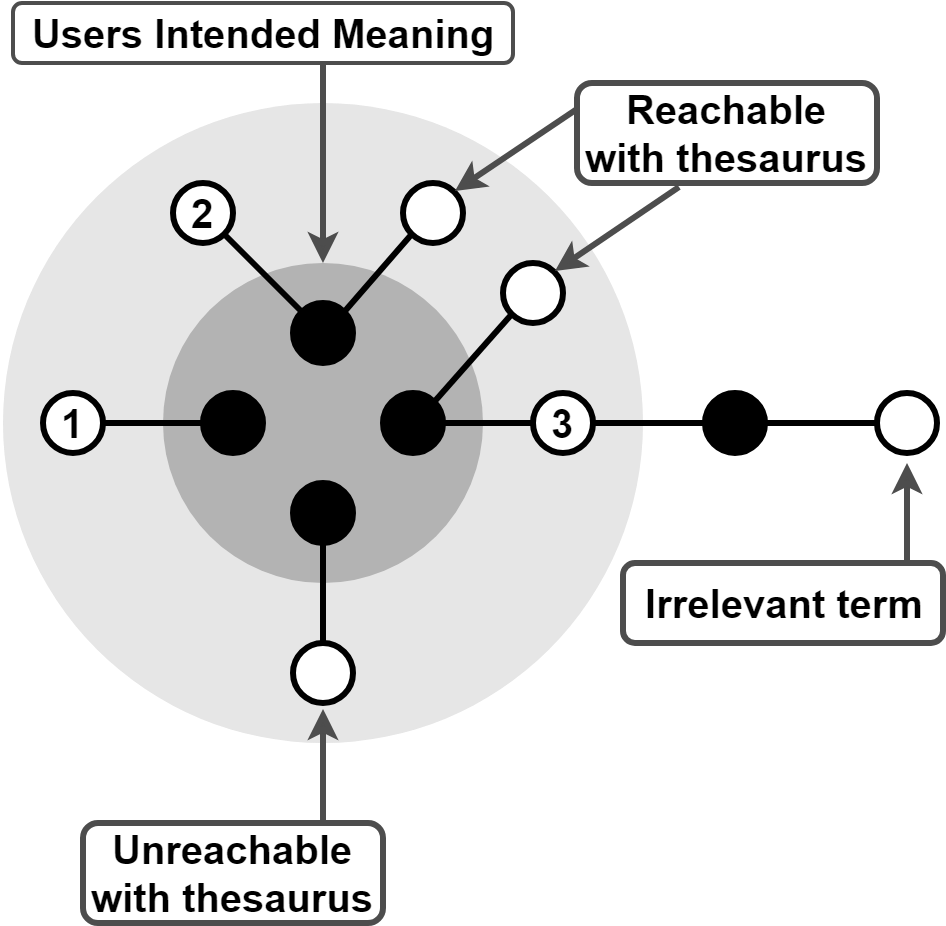
\includegraphics[width=0.6\linewidth]{graphics/query_semantic_space_labels.png}
% \caption{Query terms: 1, 2 and 3. Their SynSets (black circles) in a shared space.}
% \label{fig:querydiagram}
% \end{figure}

\begin{figure}
    \centering
    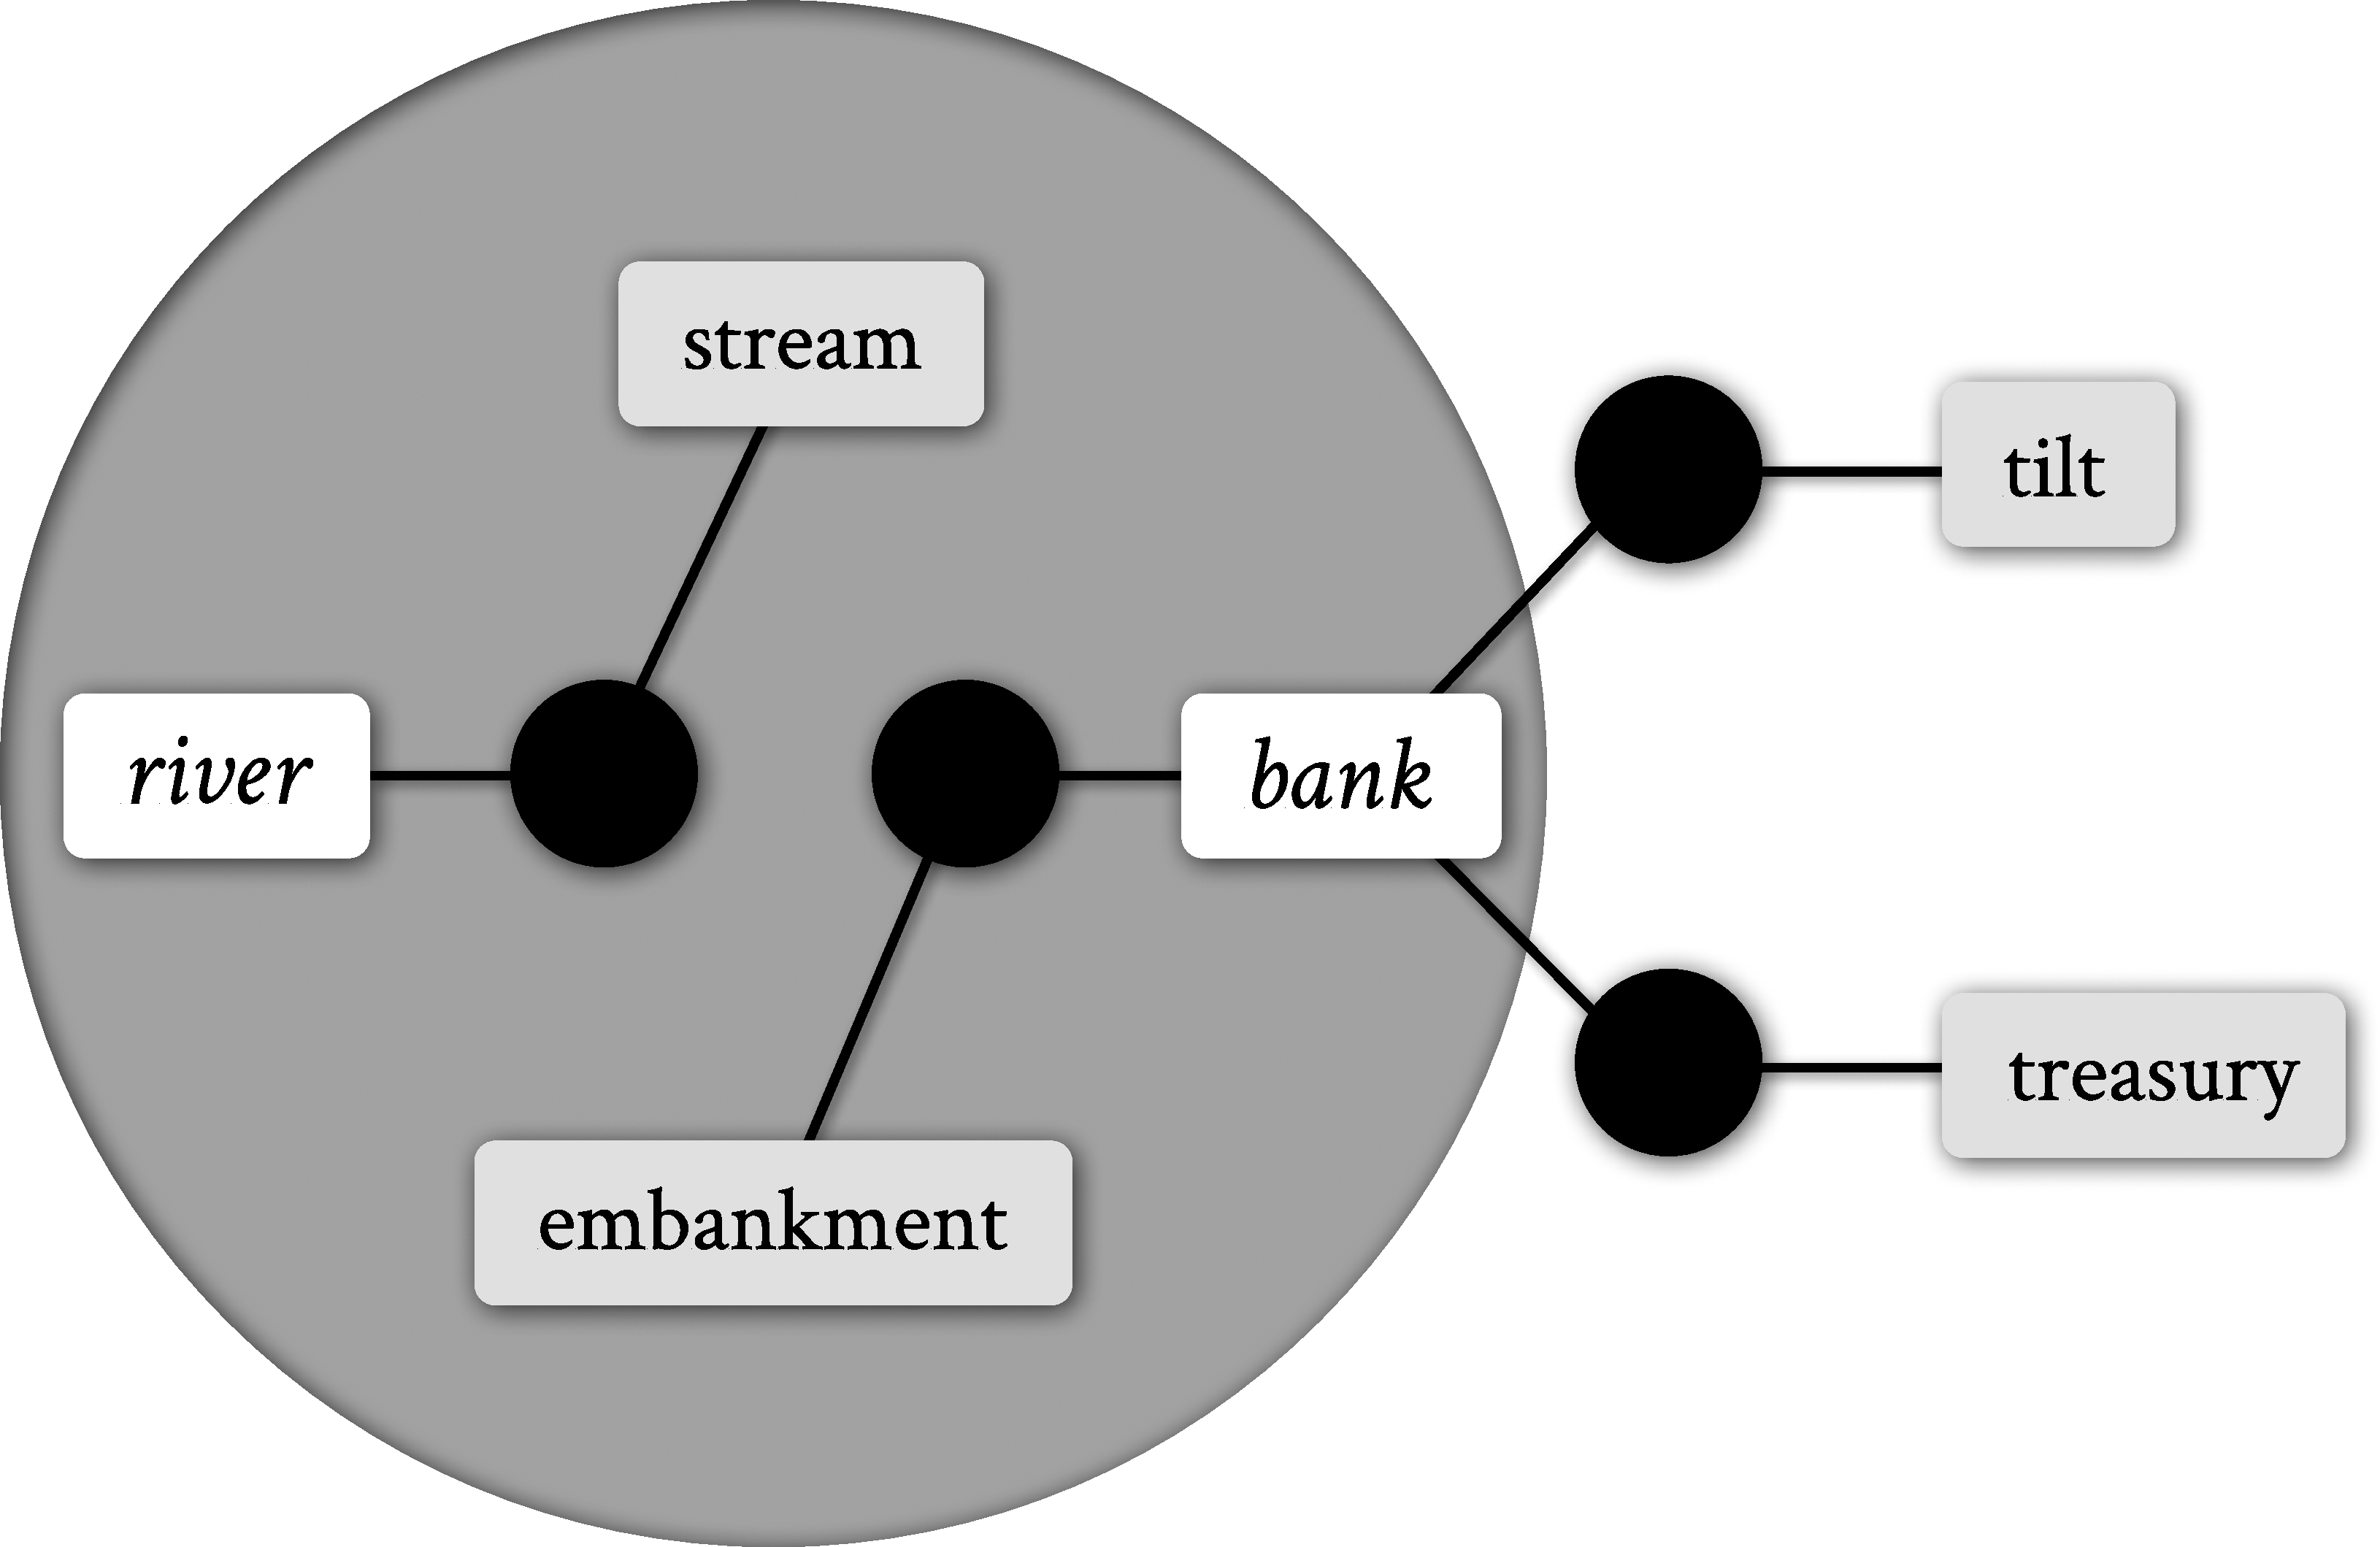
\includegraphics[width=0.7\linewidth]{graphics/concept-space.pdf}
    \caption{Concept space for query terms $Q = \{river, bank\}$ and potential expansion terms $E_Q = \{stream, embankment, tilt, treasury\}$. Black circles are SynSets with edges representing term membership. The grey circle represents the shared concept space, the user's intended meaning.}
    \label{fig:conceptspace}
\end{figure}

Figure \ref{fig:conceptspace} is an example query $Q = \{river, bank\}$, showing the relationship between the query terms, expansion terms, and SynSets, similar to Figure \ref{fig:sense-relations}. The terms and SynSets are superimposed into a conceptual space representing the user's intended meaning, their information need. The query term ``river'' is not polysemous, it's a member of one SynSet. However, bank is a member of 3 SynSets, two of which are located outside the concept space which would lead to query drift if included in the expanded query. No tournament would be necessary for ``river'', however ``bank'' requires a tournament to find the best SynSet for expansion, ideally the one which has ``embankment'' as a member.

% Figure \ref{fig:querydiagram} is an example query showing the relationship between terms (lexical tokens) and SynSets (word sense) similar to Figure \ref{fig:sense-relations}. The terms and SynSets are superimposed into the conceptual space of the information need; the user's intended meaning. The original query terms are identified with the white circles: 1, 2 and 3; the SynSets are black circles, with edges between showing WordNet (or other ontology) associations. The containing grey circle(s) represent the user's information need. Term 1 is a monoseme and has one associated SynSet. Term 3 is polysemous, as there are 2 SynSets; one contained within the information need and the other outside the information need, which is spurious and would cause query drift.

% Figure \ref{fig:querydiagram2} shows the proposed tournament resulting from the query \textit{``river bank"}. We can see that \textit{``river''} has 1 SynSet, so no tournament necessary. However, \textit{``bank''} has 3 SynSets, so we must determine which is the best for expansion. Clearly, the SynSets containing \textit{``tilt''} and \textit{``treasury''} are spurious for this query and the SynSet containing \textit{``embankment''} is not spurious.

% We choose a single SynSet by comparing the candidate expansion terms to the query context, i.e.\ the other SynSets. From a pairwise tournament the highest scoring SynSet is chosen as source for expansion terms.

% \begin{figure}
%     \centering
%     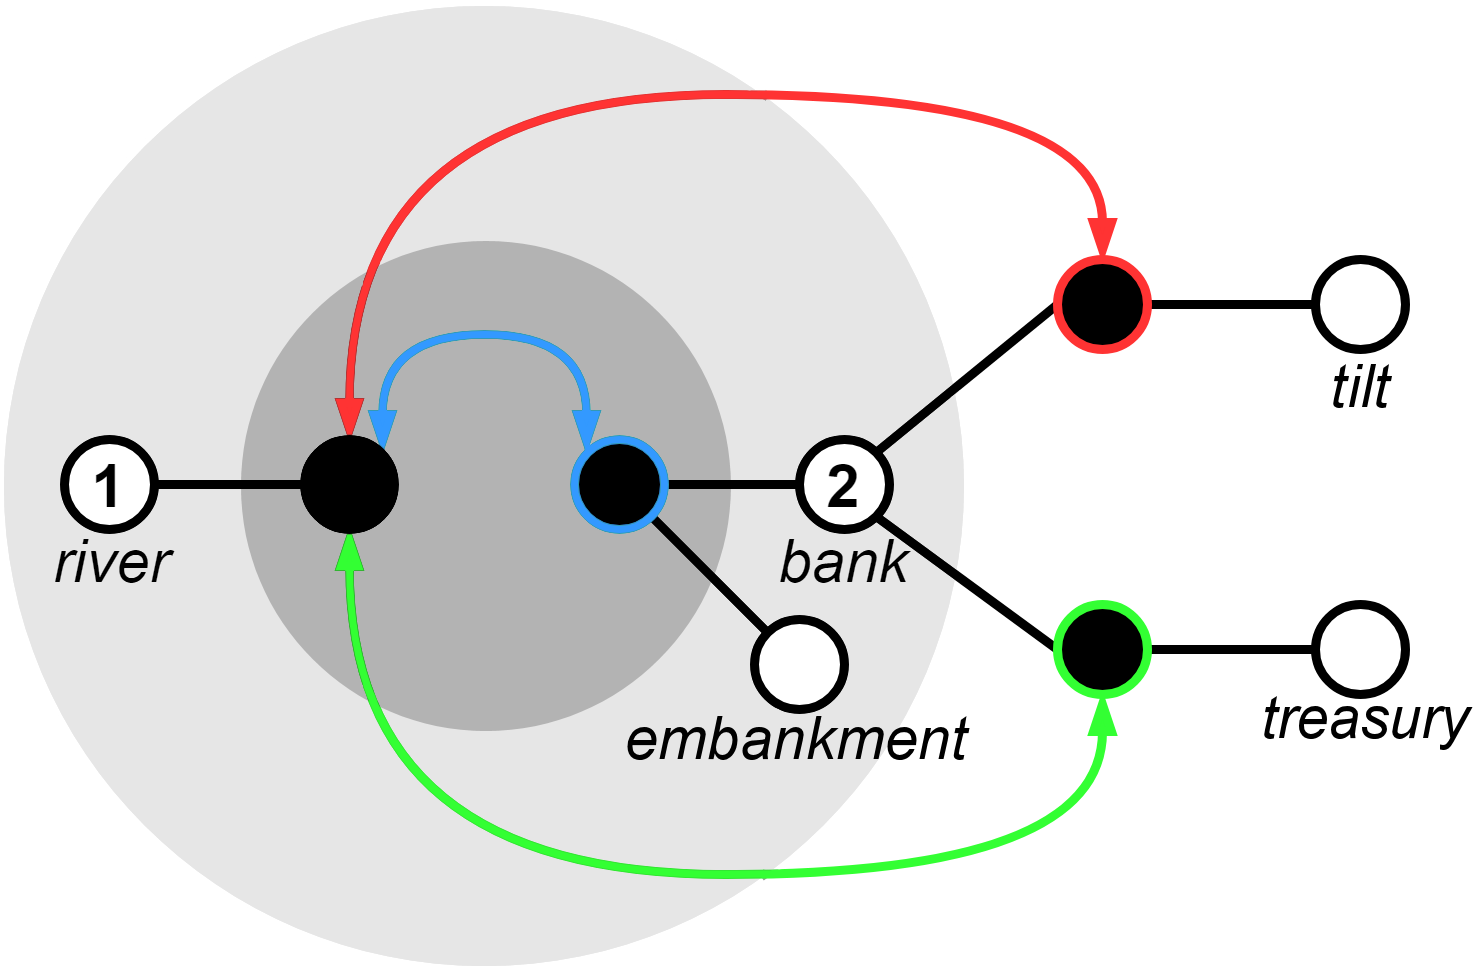
\includegraphics[width=0.6\linewidth]{graphics/tournament-2.png}
%     \caption{Tournament for the query \textit{``river bank''}}
%     \label{fig:querydiagram2}
% \end{figure}

\subsection{WordNet Structure}
We now take a closer look at the ontological structure of WordNet \cite{Miller:1995:WLD:219717.219748}.

\vspace{5pt}

\noindent \textbf{SynSet} Synonym set. A set of words that share at least one word sense, i.e.\ a single thesaurus entry.

\vspace{5pt}

\noindent \textbf{SynSets} Set of all word senses for a given term, i.e.\ potential candidates for the authors intended meaning(s). 

\vspace{5pt}

\noindent \textbf{Lemmas} Set of lexically distinct but \textit{``synonymous''} terms belonging to a SynSet.

\vspace{5pt}

% \vspace{\baselineskip}

% \noindent\textbf{Term}
% A string of characters. Can exist independent of meaning.
% \noindent\textbf{Word}
% A term authored with intended meaning, which is dependent on the context in which it was written. In rare cases, multiple meanings are simultaneously intended e.g.\ double entendre.
% \noindent\textbf{Word Sense}
% A well defined meaning associated with a term.
% \noindent\textbf{Synonyms}
% Terms that share same Word Sense.
%\noindent\textbf{Lexeme} Set of terms that share same Word Sense AND stem (e.g.\ different tenses)
%\noindent\textbf{Lemma} Canonical form or root term of a Lexeme.

\begin{figure}
    \centering
    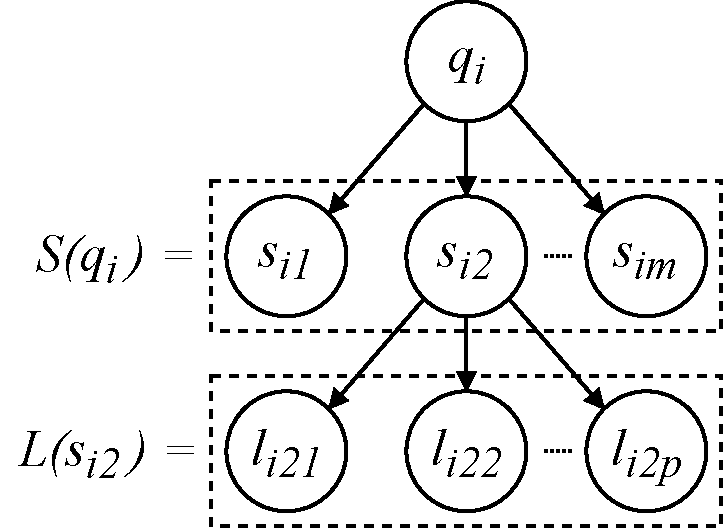
\includegraphics[width=0.6\linewidth]{graphics/lemma_diagram.pdf} 
    \caption{WordNet SynSets: ($q_i$) is the initial term; $S(q_i)$ are its SynSets, and $L(s_{ij})$ are the lexical terms contained in each SynSet.}
    \label{fig:wn}
\end{figure}

\noindent
Figure \ref{fig:wn} shows how a query term ($q_i$) associates to many SynSets ($S(q_i)$), and subsequently many more lemma terms ($L(S(q_i))$), which are used as expansion terms. If the SynSet is a reflexive relation, then one of the lemma terms ($l_{ij}$) will be lexically identical to the initial query term ($q_i$).


\subsection{The Comparison Function}
As discussed earlier, in IR, it is common to compute term similarity using the corpus statistics, e.g.\ the dice coefficient, Jaccard Index and point-wise mutual information \cite{Carpineto:2012:SAQ:2071389.2071390}. They all infer similarity from co-occurrence data, a form of \textit{syntactic similarity}. We will instead measure \textit{semantic similarity} using the structural relationships in WordNet. We will measure the similarity between SynSets by measuring the path from one SynSet to another SynSet. The supposition is that path length correlates with semantic similarity, longer paths indicate lower similarity, and shorter paths indicate higher similarity. This is clearly true for neighbours, where path length equals 1, meaning the terms share a SynSet. We will use the Wu-Palmer function \cite{Wu:1994:VSL:981732.981751}, formally defined in Equation \ref{eq:d}, to find the shortest path. Wu-Palmer also accounts for large conceptual leaps by considering the lowest common subsumer (first shared ancestor) and weighting edges according to their depth within the hierarchy such that edges between more conceptual nodes (which are closer to the root) have a higher cost. 

% Since Word Senses which are separated by a shorter path are generally more semantically similar than those with a longer path.

\begin{figure}
    \begin{flalign}
        & & distance(a, b) & = \frac{2 * depth(LCS(a, b))}{depth(a) * depth(b)} & \label{eq:d} \\
        & & LCS(a, b) & = \text{Least Common Subsumer} & \label{eq:e} \\
        & & depth(a)  & = \text{Shortest path from root to } a & \label{eq:f}
    \end{flalign}
    \caption{Wu-Palmer distance function.}
\end{figure}

% \begin{flalign}
% &  & Q  & = \{ q_1, q_2, ... q_n \} &  & \text{Query terms}\label{eq:a} \\
% &  & S(q_i)  & = \{ s_{i1}, s_{i2}, ... s_{im} \} &  &  \text{Synonym set}\label{eq:b}\\
% &  & L(s_{ij}) & = \{ l_{ij1}, l_{ij2}, ... l_{ijp} \} &  &  \text{Lemma terms}\label{eq:c}
% \end{flalign}

% $ sim(a,b) = frac{2 * depth(LCS(a, b))}{depth(a) * depth(b)} $
% sim(a, b)  similarity
% depth(a) = shortest path from root to a
% lcs(a, b) = lowest common subsumer of a and b, (closest shared ancestor).

% We will refer to the term being expanded as the \textit{term of interest}, and the set of remaining terms from the original query as the \textit{other terms}. 

\subsection{The Tournament}
The SynSets for each query term will be compared to the SynSets of the other terms using Wu-Palmer distance as the comparison function. The highest scoring SynSet wins the tournament and is chosen as the most likely candidate for the intended word sense. Then each of the lemma terms from the winning SynSet are added to the modified query. This process is repeated for each term in the original query. The algorithmic complexity of this process is exponential with respect to the number of query terms and the number of associated SynSets. However, in practice, the performance is reasonable since queries are short (see Section \ref{problems-with-relevance-models}) and the number of SynSets are small (except in the rare case of hyper-polysemous words like \textit{``set''}).

\subsubsection{A Successful Example}
%\begin{displayquote}
For the query $Q_1 = \{``river '', ``bank''\}$, \textit{``river''} has only 1 SynSet, and \textit{``bank''} has 18. Therfore, only 18 comparisons need to be made. Our method correctly identifies the SynSets:

\vspace{5pt}

\noindent
\textbf{river} \textit{``a large natural stream of water (larger than a creek)''} 

\vspace{5pt}

\noindent
\textbf{bank} \textit{``sloping land (especially the slope beside a body of water)''}

\vspace{5pt}

\noindent
This suggests that the Wu-Palmer distance function is capable for our use case.

% Supposition is that the query terms correlate e.g. ball -> pool cue -> pool
% Disamguiate ball from beach ball, or formal dance


% re explain the experiment ? ATIRE TREC...

\subsubsection{An Unsuccessful Example}

\noindent For the query $Q_2 = \{``pool '', ``cue''\}$, \textit{``pool''} has 11 SynSets, and \textit{``cue''} has 5. Therefore, 55 comparisons need to be made. The SynSets identified by our method are:

\vspace{5pt}

\noindent
\textbf{pool} \textit{``an excavation that is (usually) filled with water''}

\vspace{5pt}

\noindent
\textbf{cue} \textit{``sports implement consisting of a tapering rod used to strike a cue ball in pool or billiards.''}
% \vspace{\baselineskip}

\vspace{5pt}

\noindent
Our method failed for \textit{``pool''}, suggesting this method is not perfect in every case.

\section{Results}
% Parameters chosen Top 17 documents, top 5 terms.
Table \ref{table:results} shows our results on the TREC ad-hoc retrieval tracks. Included for comparison is a baseline (\textit{None}), which is no expansion, and the benchmark blind relevance feedback (\textit{RF}). Bold entries indicate the best result for the track. The main results from our experiments are labelled \textit{All-SynSets} (the standard approach described in Section \ref{standardTS}), and \textit{One-SynSet} (our improved method described in Section \ref{betterTS}). We also included two separate query reformulation techniques. The na{\"i}ve approach of appending terms directly to the query and term-frequency-merging (\textit{tfm}) \cite{Crimp:2017:ATR:3166072.3166074} described in Chapter \ref{chap:tfm}. Term-frequency merging attempts to reduce query drift caused by uneven numbers of expansion terms, which should be less of a problem for the \textit{One-SynSet} case.

The results are promising, as can be seen in Table \ref{table:results}. The standard approach \textit{All-SynSets} with \textit{na{\"i}ve QE} only beats the baseline in one case (TREC-6). In comparison, our method \textit{One-SynSet} with \textit{na{\"i}ve QE} improves upon the baseline in all but one case (TREC-6). And \textit{One-SynSet} with \textit{tf-merging} beats the baseline in all cases. Blind relevance feedback is still a strong contender as it remains unbeaten in TREC-1, TREC-2 and TREC-3.

%This is clear from the results, as \textit{All SynSets} was the best choice in TREC-5, TREC-6 and TREC-8. Even though this method includes many spurious terms, it's guaranteed to include a few relevant terms.

We calculated two-tailed $t$-tests on the 400 paired MAP samples. Comparing the baseline against, All-Synsets, and One-SynSet, and in every case, we obtained $p$-values $< 0.05$, which suggests that the observed differences cannot be attributed to chance alone.

% none vs onesynset_lemma = 0.01128541
% none vs all_synset_head_word = 0.5462267


%For each query term, we take every possible Word Sense, and for every possible 

%two terms to distinguish the two different modes, for expansion term selection

%1) All SynSets 
%2) One SynSet

%restricted term selection using information from the query context

%query context informs expansion term selection




\begin{table*}[h]
\centering
\resizebox{\textwidth}{!}{
\begin{tabular}{|l|l|r|r|r|r|r|r|r|r|}
\hline
Term Selection  & Expansion     & TREC-1          & TREC-2          & TREC-3          & TREC-4          & TREC-5          & TREC-6          & TREC-7          & TREC-8          \\ \hline \hline
None            & N/A              & 0.2181          & 0.1993          & 0.2324          & 0.1727          & 0.1432          & 0.1891          & 0.1905          & 0.2195          \\
RF              & na{\"i}ve QE         & \textbf{0.2601} & \textbf{0.2521} & \textbf{0.2988} & 0.2041          & 0.1369          & 0.1646          & 0.2185          & 0.2460          \\ \hline
All-SynSets       & na{\"i}ve QE     & 0.2128          & 0.1961          & 0.2243          & 0.1265          & 0.1327          & 0.2041          & 0.1822          & 0.2187          \\
One-SynSet               & na{\"i}ve QE     & 0.2318          & 0.2104          & 0.2398          & 0.2101          & 0.1476          & 0.1781          & 0.2163          & 0.2301          \\ \hline
All-SynSets       & tfm           & 0.2323          & 0.2095          & 0.2379          & 0.1721          & \textbf{0.1618} & \textbf{0.2214} & 0.1953          & \textbf{0.2440} \\ 
One-SynSet               & tfm           & 0.2380          & 0.2286          & 0.2529          & \textbf{0.2179} & 0.1537          & 0.2007          & \textbf{0.2211} & 0.2310          \\ \hline
\end{tabular}
}
% \caption{Mean Average Precision Across TREC 1-8}
\caption{Comparing the MAP of our (One-SynSet) method to the standard (All-SynSets) method. With no expansion (None) as a baseline and relevance feedback (RF) as a benchmark. Across 8 TREC tracks, bold entries are the top result. $t$-tests between each of the 400 paired MAP samples produced $p$-values $< 0.05$.}
\label{table:results}
\end{table*}


\subsection{Failure Analysis}

%Including expansion terms from all SynSets does improve query performance x percent of the time. 

%Which suggests that the centroid of the query is 
If we look at the results for TREC-7 query 2: \textit{``british chunnel impact''} in Table \ref{table:T-7-2-map}, we can see that our method has an enormously positive impact. This is partly because it only includes 8 extra terms from 3 SynSets (one for each term), instead of the na{\"i}ve All-Synset approach, which includes 21 terms from 9 different SynSets causing significant query drift. More specifically, the lemma terms from \textit{impact} include \textit{``touch, bear, shock''}, which causes significant query drift in the All-SynSet case.

\begin{table}[h]
\centering
\begin{tabular}{|l|l|l|}
\hline
Term selection  & Expansion  & AP      \\ \hline
None (baseline) &            & 0.0513 \\
All-SynSets     & appending  & 0.0421 \\
All-SynSets     & tf-merging & 0.0509 \\
One-SynSet      & appending  & 0.3118 \\
One-SynSet      & tf-merging & 0.2045 \\ \hline
\end{tabular}
\caption{TREC-7 query 2 Average Precision}
\label{table:T-7-2-map}
\end{table}

%\begin{table}[h]
%\centering
%\caption{TREC-7 query 2 Expansion Terms for \textit{``impact''}}
%\label{table:T-7-2-expansions}
%\begin{tabular}{|l|llll|}
%\hline
%All-SynSets & impact & affect       & bear        & upon \\ \hline
%One-SynSet  & impact & encroachment & impengement &      \\ \hline
%\end{tabular}
%\end{table}

However, if we look at TREC-7 query 15 in Table \ref{table:T-7-15-map}, \textit{``el nino''}, our method is ineffective. Inspecting the expansion terms chosen, shown in Table \ref{table:T-7-15-expansions}, we can see that the term \textit{``el''} is incorrectly identified as the \textit{Chicago ``L'' Train}. This example is particularly bad as \textit{``el nino''} is a recent loan word from Spanish which does not yet exist in WordNet.

\begin{table}[h]
\centering
\begin{tabular}{|l|l|l|}
\hline
Term selection  & Expansion  & AP      \\ \hline
None (baseline) &            & 0.7861 \\
All-SynSets     & appending  & 0.7843 \\
All-SynSets     & tf-merging & 0.8466 \\
One-SynSet      & appending  & 0.1947 \\
One-SynSet      & tf-merging & 0.8120 \\ \hline
\end{tabular}
\caption{TREC-7 query 15 Average Precision}
\label{table:T-7-15-map}
\end{table}

\begin{table}[h]
\centering
\begin{tabular}{|l|lllll|}
\hline
All-SynSets & alt & altitude & el       & elevation & ...        \\ \hline
One-SynSet  & el  & elevated & railroad  & railway & ... \\ \hline
\end{tabular}
\caption{Some expansion for the query term \textit{``el''}, in TREC-7 query 15}
\label{table:T-7-15-expansions}
\end{table}

% \subsection{Using the Similarity Score as a Predictor}
% The larger the similarity score, the more relevant the SynSet is assumed to be. So it is obvious to try and use the similarity score to predict the improvement of the modified query. Measuring the correlation using the Pearson bivariate method gives a score of approximately 0 ( precisely $-0.0617$ ). This suggests \textit{no} simple correlation between the \textit{Wu-Palmer Similarity Score} and the \textit{Mean Average Precision improvement (from the baseline)}. 

%It seems the score is tightly linked to the terms it is computed from. Because even a winning score from a tournament can be relatively small (compared to other tournaments) and yet, it can still improve the query. And occasionally a really large score will fail to improve a query, by misidentifying the intended Word Sense.

\section{Future Work}
Our method is essentially performing word sense disambiguation on polysemes where SynSets are treated as \textit{word sense}. There is still no assurance that our method correctly identifies the intended word sense of the original query term(s) as it is limited by the semantics of the query context. It still ignores many other features like syntactic grammar.

Our current method could, for example, select a noun-SynSet for a query term that is grammatically a verb. WordNet provides \textit{part of speech} tagging by indicating which lexical category the SynSet belongs to (e.g.\ noun, verb, adjective, etc.). Accounting for the lexical category could improve our results, but it would require the queries to be written with correct syntactic grammar, which is not guaranteed.

% \cite{Voorhees:1994:QEU:188490.188508}

The Wu-Palmer distance function is a pair-wise comparison and is ideal for queries with only 2 terms. For longer queries, a tournament of comparisons is needed, but performing a group-wise comparison directly would be more appropriate, like the group-wise Jaccard Index or the group-wise Resnik comparison \cite{Manda327833}. Comparisons of SynSets within WordNet is based on finding the shortest path in the graph. A group-wise comparison would be equivalent to finding the minimal subgraph that includes at least one SynSet from each query term. This subgraph would be a tree since a minimal graph has no cycles. The tree's intermediary nodes (SynSets) used to construct the tree could also be used for expansion terms. This can be described as a variant of the Prize Collecting Steiner tree problem \cite{Johnson:2000:PCS:338219.338637}, where we would minimize edge cost and maximize vertex profit. 

% In our case, profit would be indicated by \textit{stop words} having small values and \textit{content bearing terms} having high values. This is an NP-hard problem.

\section{Conclusions}
Overall, our results are promising. Blind relevance feedback remains a strong option as it can find expansion terms that are not semantically related to any of the original query terms, i.e.\ it can include related concept(s) that the user did not think to include, which is beyond the scope of vocabulary mismatch.

Using our query context informed method, we refined the expansion terms obtained from a thesaurus, which is more effective than using a thesaurus blindly. Term frequency merging was able to be applied to both methods and improved them in all cases. 

% We assumed that WordNet is sufficiently complete

% We also assumed that lemma terms would exist at the same level



